\documentclass[1p]{elsarticle_modified}
%\bibliographystyle{elsarticle-num}

%\usepackage[colorlinks]{hyperref}
%\usepackage{abbrmath_seonhwa} %\Abb, \Ascr, \Acal ,\Abf, \Afrak
\usepackage{amsfonts}
\usepackage{amssymb}
\usepackage{amsmath}
\usepackage{amsthm}
\usepackage{scalefnt}
\usepackage{amsbsy}
\usepackage{kotex}
\usepackage{caption}
\usepackage{subfig}
\usepackage{color}
\usepackage{graphicx}
\usepackage{xcolor} %% white, black, red, green, blue, cyan, magenta, yellow
\usepackage{float}
\usepackage{setspace}
\usepackage{hyperref}

\usepackage{tikz}
\usetikzlibrary{arrows}

\usepackage{multirow}
\usepackage{array} % fixed length table
\usepackage{hhline}

%%%%%%%%%%%%%%%%%%%%%
\makeatletter
\renewcommand*\env@matrix[1][\arraystretch]{%
	\edef\arraystretch{#1}%
	\hskip -\arraycolsep
	\let\@ifnextchar\new@ifnextchar
	\array{*\c@MaxMatrixCols c}}
\makeatother %https://tex.stackexchange.com/questions/14071/how-can-i-increase-the-line-spacing-in-a-matrix
%%%%%%%%%%%%%%%

\usepackage[normalem]{ulem}

\newcommand{\msout}[1]{\ifmmode\text{\sout{\ensuremath{#1}}}\else\sout{#1}\fi}
%SOURCE: \msout is \stkout macro in https://tex.stackexchange.com/questions/20609/strikeout-in-math-mode

\newcommand{\cancel}[1]{
	\ifmmode
	{\color{red}\msout{#1}}
	\else
	{\color{red}\sout{#1}}
	\fi
}

\newcommand{\add}[1]{
	{\color{blue}\uwave{#1}}
}

\newcommand{\replace}[2]{
	\ifmmode
	{\color{red}\msout{#1}}{\color{blue}\uwave{#2}}
	\else
	{\color{red}\sout{#1}}{\color{blue}\uwave{#2}}
	\fi
}

\newcommand{\Sol}{\mathcal{S}} %segment
\newcommand{\D}{D} %diagram
\newcommand{\A}{\mathcal{A}} %arc


%%%%%%%%%%%%%%%%%%%%%%%%%%%%%5 test

\def\sl{\operatorname{\textup{SL}}(2,\Cbb)}
\def\psl{\operatorname{\textup{PSL}}(2,\Cbb)}
\def\quan{\mkern 1mu \triangleright \mkern 1mu}

\theoremstyle{definition}
\newtheorem{thm}{Theorem}[section]
\newtheorem{prop}[thm]{Proposition}
\newtheorem{lem}[thm]{Lemma}
\newtheorem{ques}[thm]{Question}
\newtheorem{cor}[thm]{Corollary}
\newtheorem{defn}[thm]{Definition}
\newtheorem{exam}[thm]{Example}
\newtheorem{rmk}[thm]{Remark}
\newtheorem{alg}[thm]{Algorithm}

\newcommand{\I}{\sqrt{-1}}
\begin{document}

%\begin{frontmatter}
%
%\title{Boundary parabolic representations of knots up to 8 crossings}
%
%%% Group authors per affiliation:
%\author{Yunhi Cho} 
%\address{Department of Mathematics, University of Seoul, Seoul, Korea}
%\ead{yhcho@uos.ac.kr}
%
%
%\author{Seonhwa Kim} %\fnref{s_kim}}
%\address{Center for Geometry and Physics, Institute for Basic Science, Pohang, 37673, Korea}
%\ead{ryeona17@ibs.re.kr}
%
%\author{Hyuk Kim}
%\address{Department of Mathematical Sciences, Seoul National University, Seoul 08826, Korea}
%\ead{hyukkim@snu.ac.kr}
%
%\author{Seokbeom Yoon}
%\address{Department of Mathematical Sciences, Seoul National University, Seoul, 08826,  Korea}
%\ead{sbyoon15@snu.ac.kr}
%
%\begin{abstract}
%We find all boundary parabolic representation of knots up to 8 crossings.
%
%\end{abstract}
%\begin{keyword}
%    \MSC[2010] 57M25 
%\end{keyword}
%
%\end{frontmatter}

%\linenumbers
%\tableofcontents
%
\newcommand\colored[1]{\textcolor{white}{\rule[-0.35ex]{0.8em}{1.4ex}}\kern-0.8em\color{red} #1}%
%\newcommand\colored[1]{\textcolor{white}{ #1}\kern-2.17ex	\textcolor{white}{ #1}\kern-1.81ex	\textcolor{white}{ #1}\kern-2.15ex\color{red}#1	}

{\Large $\underline{12n_{0334}~(K12n_{0334})}$}

\setlength{\tabcolsep}{10pt}
\renewcommand{\arraystretch}{1.6}
\vspace{1cm}\begin{tabular}{m{100pt}>{\centering\arraybackslash}m{274pt}}
\multirow{5}{120pt}{
	\centering
	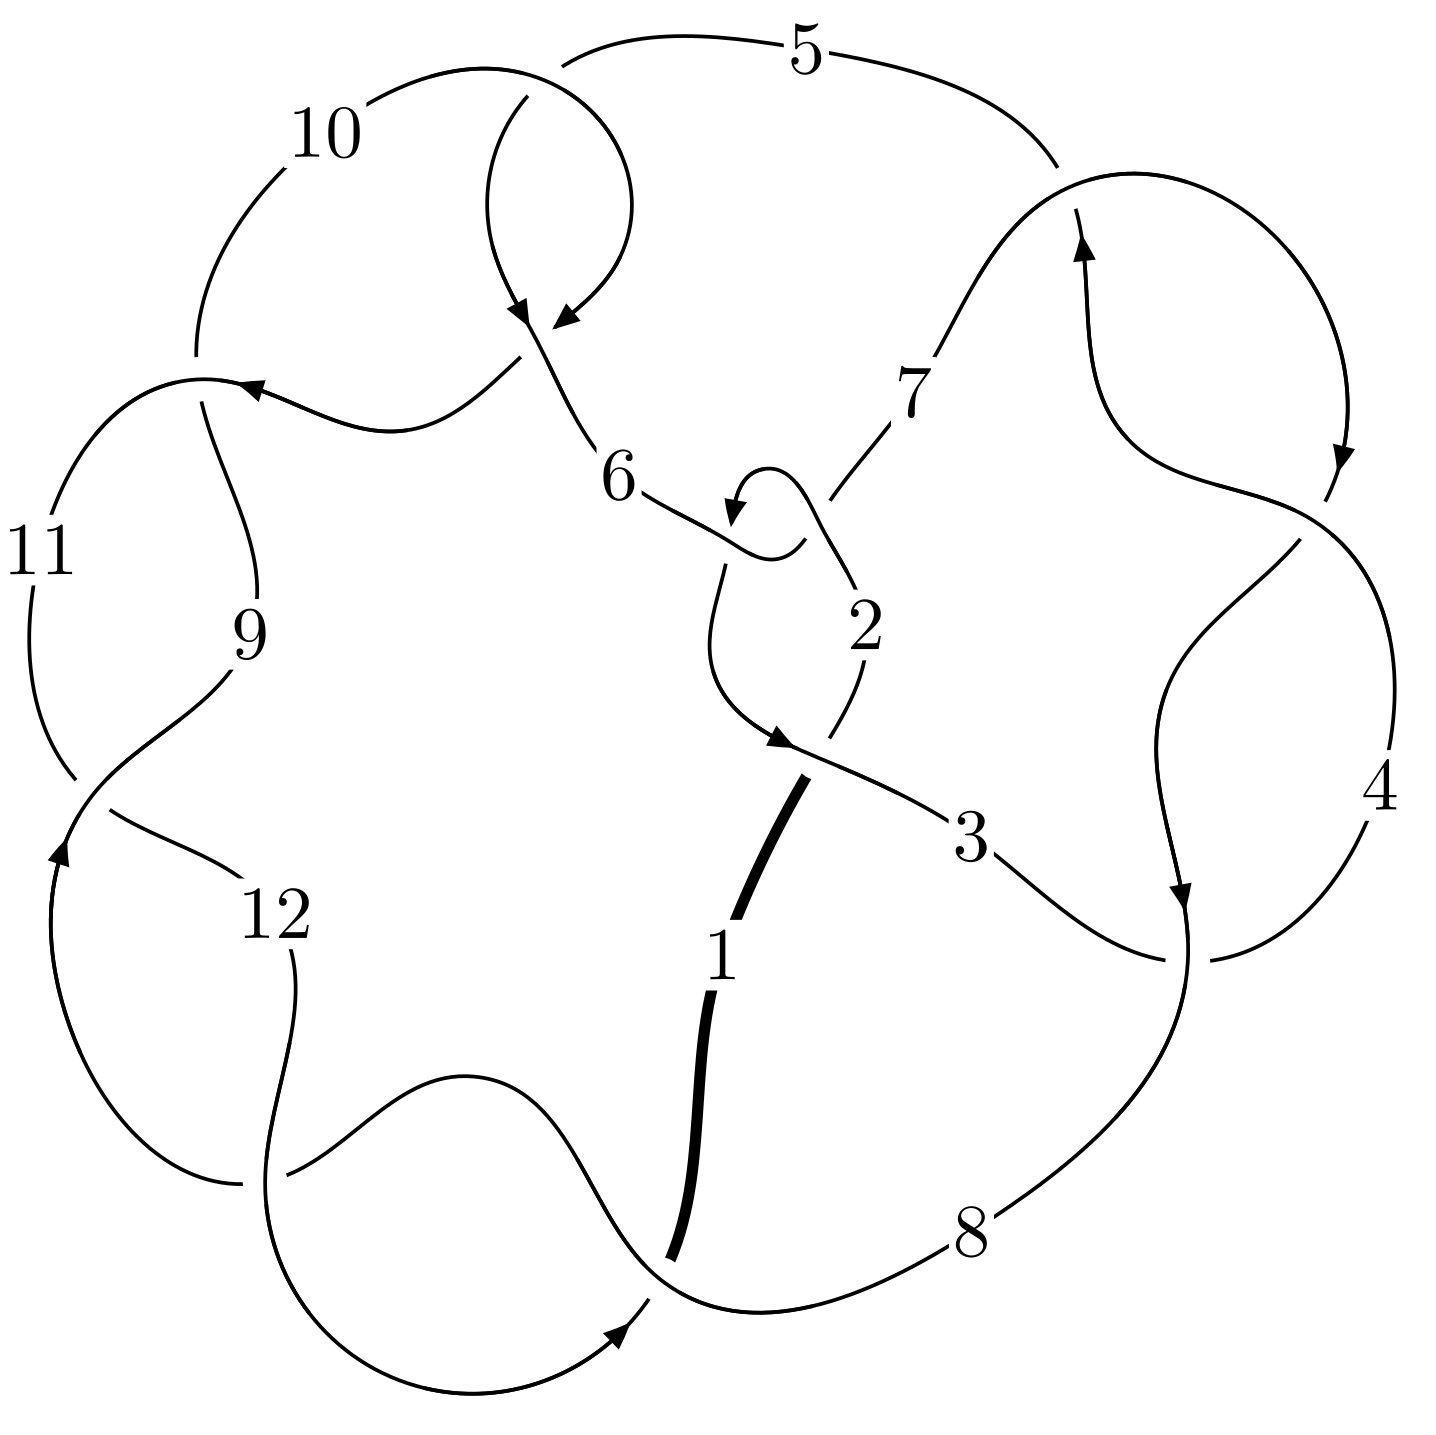
\includegraphics[width=112pt]{../../../GIT/diagram.site/Diagrams/png/2423_12n_0334.png}\\
\ \ \ A knot diagram\footnotemark}&
\allowdisplaybreaks
\textbf{Linearized knot diagam} \\
\cline{2-2}
 &
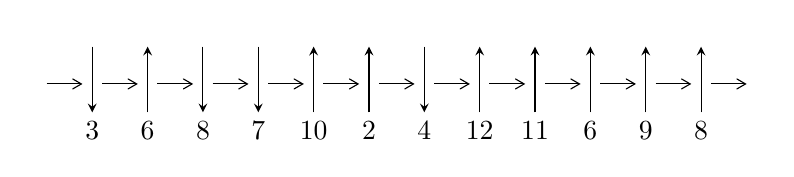
\begin{tikzpicture}[x=20pt, y=17pt]
	% nodes
	\node (C0) at (0, 0) {};
	\node (C1) at (1, 0) {};
	\node (C1U) at (1, +1) {};
	\node (C1D) at (1, -1) {3};

	\node (C2) at (2, 0) {};
	\node (C2U) at (2, +1) {};
	\node (C2D) at (2, -1) {6};

	\node (C3) at (3, 0) {};
	\node (C3U) at (3, +1) {};
	\node (C3D) at (3, -1) {8};

	\node (C4) at (4, 0) {};
	\node (C4U) at (4, +1) {};
	\node (C4D) at (4, -1) {7};

	\node (C5) at (5, 0) {};
	\node (C5U) at (5, +1) {};
	\node (C5D) at (5, -1) {10};

	\node (C6) at (6, 0) {};
	\node (C6U) at (6, +1) {};
	\node (C6D) at (6, -1) {2};

	\node (C7) at (7, 0) {};
	\node (C7U) at (7, +1) {};
	\node (C7D) at (7, -1) {4};

	\node (C8) at (8, 0) {};
	\node (C8U) at (8, +1) {};
	\node (C8D) at (8, -1) {12};

	\node (C9) at (9, 0) {};
	\node (C9U) at (9, +1) {};
	\node (C9D) at (9, -1) {11};

	\node (C10) at (10, 0) {};
	\node (C10U) at (10, +1) {};
	\node (C10D) at (10, -1) {6};

	\node (C11) at (11, 0) {};
	\node (C11U) at (11, +1) {};
	\node (C11D) at (11, -1) {9};

	\node (C12) at (12, 0) {};
	\node (C12U) at (12, +1) {};
	\node (C12D) at (12, -1) {8};
	\node (C13) at (13, 0) {};

	% arrows
	\draw[->,>={angle 60}]
	(C0) edge (C1) (C1) edge (C2) (C2) edge (C3) (C3) edge (C4) (C4) edge (C5) (C5) edge (C6) (C6) edge (C7) (C7) edge (C8) (C8) edge (C9) (C9) edge (C10) (C10) edge (C11) (C11) edge (C12) (C12) edge (C13) ;	\draw[->,>=stealth]
	(C1U) edge (C1D) (C2D) edge (C2U) (C3U) edge (C3D) (C4U) edge (C4D) (C5D) edge (C5U) (C6D) edge (C6U) (C7U) edge (C7D) (C8D) edge (C8U) (C9D) edge (C9U) (C10D) edge (C10U) (C11D) edge (C11U) (C12D) edge (C12U) ;
	\end{tikzpicture} \\
\hhline{~~} \\& 
\textbf{Solving Sequence} \\ \cline{2-2} 
 &
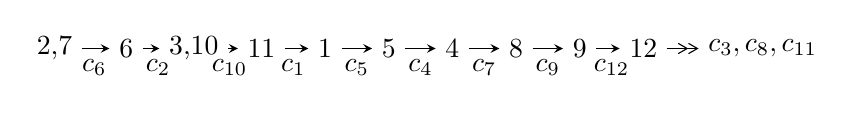
\begin{tikzpicture}[x=23pt, y=7pt]
	% node
	\node (A0) at (-1/8, 0) {2,7};
	\node (A1) at (1, 0) {6};
	\node (A2) at (33/16, 0) {3,10};
	\node (A3) at (25/8, 0) {11};
	\node (A4) at (33/8, 0) {1};
	\node (A5) at (41/8, 0) {5};
	\node (A6) at (49/8, 0) {4};
	\node (A7) at (57/8, 0) {8};
	\node (A8) at (65/8, 0) {9};
	\node (A9) at (73/8, 0) {12};
	\node (C1) at (1/2, -1) {$c_{6}$};
	\node (C2) at (3/2, -1) {$c_{2}$};
	\node (C3) at (21/8, -1) {$c_{10}$};
	\node (C4) at (29/8, -1) {$c_{1}$};
	\node (C5) at (37/8, -1) {$c_{5}$};
	\node (C6) at (45/8, -1) {$c_{4}$};
	\node (C7) at (53/8, -1) {$c_{7}$};
	\node (C8) at (61/8, -1) {$c_{9}$};
	\node (C9) at (69/8, -1) {$c_{12}$};
	\node (A10) at (11, 0) {$c_{3},c_{8},c_{11}$};

	% edge
	\draw[->,>=stealth]	
	(A0) edge (A1) (A1) edge (A2) (A2) edge (A3) (A3) edge (A4) (A4) edge (A5) (A5) edge (A6) (A6) edge (A7) (A7) edge (A8) (A8) edge (A9) ;
	\draw[->>,>={angle 60}]	
	(A9) edge (A10);
\end{tikzpicture} \\ 

\end{tabular} \\

\footnotetext{
The image of knot diagram is generated by the software ``\textbf{Draw programme}" developed by Andrew Bartholomew(\url{http://www.layer8.co.uk/maths/draw/index.htm\#Running-draw}), where we modified some parts for our purpose(\url{https://github.com/CATsTAILs/LinksPainter}).
}\phantom \\ \newline 
\centering \textbf{Ideals for irreducible components\footnotemark of $X_{\text{par}}$} 
 
\begin{align*}
I^u_{1}&=\langle 
-1.23152\times10^{16} u^{29}+1.53695\times10^{16} u^{28}+\cdots+5.84790\times10^{16} b-9.74776\times10^{15},\\
\phantom{I^u_{1}}&\phantom{= \langle  }-4.32154\times10^{16} u^{29}+2.87372\times10^{16} u^{28}+\cdots+1.16958\times10^{17} a-5.09997\times10^{16},\;u^{30}- u^{29}+\cdots+7 u+2\rangle \\
I^u_{2}&=\langle 
9 a^3 u+23 a^3- a^2 u+11 a^2+57 a u+61 b+105 a-66 u-6,\;a^4- a^3 u+2 a^2 u+3 a^2-5 a u- a+2 u-3,\\
\phantom{I^u_{2}}&\phantom{= \langle  }u^2+1\rangle \\
I^u_{3}&=\langle 
u^8- u^7+2 u^6-2 u^5+u^4- u^3+u^2+b- u,\;u^7+u^6+2 u^5+2 u^4+u^3+u^2+a+u+1,\\
\phantom{I^u_{3}}&\phantom{= \langle  }u^9+3 u^7- u^6+3 u^5-2 u^4+3 u^3- u^2+2 u-1\rangle \\
\\
\end{align*}
\raggedright * 3 irreducible components of $\dim_{\mathbb{C}}=0$, with total 47 representations.\\
\footnotetext{All coefficients of polynomials are rational numbers. But the coefficients are sometimes approximated in decimal forms when there is not enough margin.}
\newpage
\renewcommand{\arraystretch}{1}
\centering \section*{I. $I^u_{1}= \langle -1.23\times10^{16} u^{29}+1.54\times10^{16} u^{28}+\cdots+5.85\times10^{16} b-9.75\times10^{15},\;-4.32\times10^{16} u^{29}+2.87\times10^{16} u^{28}+\cdots+1.17\times10^{17} a-5.10\times10^{16},\;u^{30}- u^{29}+\cdots+7 u+2 \rangle$}
\flushleft \textbf{(i) Arc colorings}\\
\begin{tabular}{m{7pt} m{180pt} m{7pt} m{180pt} }
\flushright $a_{2}=$&$\begin{pmatrix}0\\u\end{pmatrix}$ \\
\flushright $a_{7}=$&$\begin{pmatrix}1\\0\end{pmatrix}$ \\
\flushright $a_{6}=$&$\begin{pmatrix}1\\u^2\end{pmatrix}$ \\
\flushright $a_{3}=$&$\begin{pmatrix}u\\u^3+u\end{pmatrix}$ \\
\flushright $a_{10}=$&$\begin{pmatrix}0.369495 u^{29}-0.245705 u^{28}+\cdots+14.2746 u+0.436051\\0.210593 u^{29}-0.262820 u^{28}+\cdots+3.53091 u+0.166688\end{pmatrix}$ \\
\flushright $a_{11}=$&$\begin{pmatrix}0.672620 u^{29}-0.609580 u^{28}+\cdots+19.4110 u+0.850319\\0.211783 u^{29}-0.281668 u^{28}+\cdots+3.34990 u+0.288187\end{pmatrix}$ \\
\flushright $a_{1}=$&$\begin{pmatrix}u^3\\u^5+u^3+u\end{pmatrix}$ \\
\flushright $a_{5}=$&$\begin{pmatrix}-0.688243 u^{29}+0.596482 u^{28}+\cdots-22.1445 u-4.75119\\-0.0998548 u^{29}+0.00973725 u^{28}+\cdots-4.79516 u-0.887435\end{pmatrix}$ \\
\flushright $a_{4}=$&$\begin{pmatrix}-0.788098 u^{29}+0.606219 u^{28}+\cdots-26.9397 u-5.63863\\-0.0998548 u^{29}+0.00973725 u^{28}+\cdots-4.79516 u-0.887435\end{pmatrix}$ \\
\flushright $a_{8}=$&$\begin{pmatrix}0.625597 u^{29}-0.813840 u^{28}+\cdots+3.22541 u-3.26533\\0.0901176 u^{29}-0.131952 u^{28}+\cdots+0.188451 u-1.19971\end{pmatrix}$ \\
\flushright $a_{9}=$&$\begin{pmatrix}0.772220 u^{29}-1.17415 u^{28}+\cdots-1.69794 u-6.69657\\0.193509 u^{29}-0.293937 u^{28}+\cdots-0.448992 u-0.953828\end{pmatrix}$ \\
\flushright $a_{12}=$&$\begin{pmatrix}-1.07677 u^{29}+0.793142 u^{28}+\cdots-38.8926 u-7.27684\\-0.188243 u^{29}+0.0964819 u^{28}+\cdots-7.64451 u-1.25119\end{pmatrix}$\\&\end{tabular}
\flushleft \textbf{(ii) Obstruction class $= -1$}\\~\\
\flushleft \textbf{(iii) Cusp Shapes $= \frac{6673390003312773}{9746501057251736} u^{29}-\frac{1203194374045575}{2436625264312934} u^{28}+\cdots+\frac{172887881292571847}{9746501057251736} u+\frac{53741926556471299}{4873250528625868}$}\\~\\
\newpage\renewcommand{\arraystretch}{1}
\flushleft \textbf{(iv) u-Polynomials at the component}\newline \\
\begin{tabular}{m{50pt}|m{274pt}}
Crossings & \hspace{64pt}u-Polynomials at each crossing \\
\hline $$\begin{aligned}c_{1}\end{aligned}$$&$\begin{aligned}
&u^{30}+5 u^{29}+\cdots+75 u+4
\end{aligned}$\\
\hline $$\begin{aligned}c_{2},c_{6}\end{aligned}$$&$\begin{aligned}
&u^{30}- u^{29}+\cdots+7 u+2
\end{aligned}$\\
\hline $$\begin{aligned}c_{3},c_{4},c_{7}\end{aligned}$$&$\begin{aligned}
&u^{30}- u^{29}+\cdots+13 u+2
\end{aligned}$\\
\hline $$\begin{aligned}c_{5},c_{10}\end{aligned}$$&$\begin{aligned}
&u^{30}-2 u^{29}+\cdots- u+2
\end{aligned}$\\
\hline $$\begin{aligned}c_{8},c_{9},c_{11}\\c_{12}\end{aligned}$$&$\begin{aligned}
&u^{30}-8 u^{29}+\cdots+19 u+4
\end{aligned}$\\
\hline
\end{tabular}\\~\\
\newpage\renewcommand{\arraystretch}{1}
\flushleft \textbf{(v) Riley Polynomials at the component}\newline \\
\begin{tabular}{m{50pt}|m{274pt}}
Crossings & \hspace{64pt}Riley Polynomials at each crossing \\
\hline $$\begin{aligned}c_{1}\end{aligned}$$&$\begin{aligned}
&y^{30}+49 y^{29}+\cdots-2273 y+16
\end{aligned}$\\
\hline $$\begin{aligned}c_{2},c_{6}\end{aligned}$$&$\begin{aligned}
&y^{30}+5 y^{29}+\cdots+75 y+4
\end{aligned}$\\
\hline $$\begin{aligned}c_{3},c_{4},c_{7}\end{aligned}$$&$\begin{aligned}
&y^{30}+41 y^{29}+\cdots+283 y+4
\end{aligned}$\\
\hline $$\begin{aligned}c_{5},c_{10}\end{aligned}$$&$\begin{aligned}
&y^{30}-8 y^{29}+\cdots+19 y+4
\end{aligned}$\\
\hline $$\begin{aligned}c_{8},c_{9},c_{11}\\c_{12}\end{aligned}$$&$\begin{aligned}
&y^{30}+28 y^{29}+\cdots-721 y+16
\end{aligned}$\\
\hline
\end{tabular}\\~\\
\newpage\flushleft \textbf{(vi) Complex Volumes and Cusp Shapes}
$$\begin{array}{c|c|c}  
\text{Solutions to }I^u_{1}& \I (\text{vol} + \sqrt{-1}CS) & \text{Cusp shape}\\
 \hline 
\begin{aligned}
u &= -0.698998 + 0.613459 I \\
a &= \phantom{-}2.39480 + 0.61262 I \\
b &= -0.15133 - 1.76319 I\end{aligned}
 & \phantom{-}2.77724 - 3.85593 I & \phantom{-}9.07460 + 7.10921 I \\ \hline\begin{aligned}
u &= -0.698998 - 0.613459 I \\
a &= \phantom{-}2.39480 - 0.61262 I \\
b &= -0.15133 + 1.76319 I\end{aligned}
 & \phantom{-}2.77724 + 3.85593 I & \phantom{-}9.07460 - 7.10921 I \\ \hline\begin{aligned}
u &= \phantom{-}0.011422 + 1.077760 I \\
a &= \phantom{-}0.273728 + 1.371180 I \\
b &= \phantom{-}0.555566 - 0.741416 I\end{aligned}
 & -8.36072 + 3.13944 I & -5.78917 - 2.58972 I \\ \hline\begin{aligned}
u &= \phantom{-}0.011422 - 1.077760 I \\
a &= \phantom{-}0.273728 - 1.371180 I \\
b &= \phantom{-}0.555566 + 0.741416 I\end{aligned}
 & -8.36072 - 3.13944 I & -5.78917 + 2.58972 I \\ \hline\begin{aligned}
u &= \phantom{-}0.108984 + 0.894375 I \\
a &= \phantom{-}0.301960 - 0.991096 I \\
b &= -0.689592 + 0.428612 I\end{aligned}
 & -1.44382 + 1.63203 I & -3.48932 - 5.49543 I \\ \hline\begin{aligned}
u &= \phantom{-}0.108984 - 0.894375 I \\
a &= \phantom{-}0.301960 + 0.991096 I \\
b &= -0.689592 - 0.428612 I\end{aligned}
 & -1.44382 - 1.63203 I & -3.48932 + 5.49543 I \\ \hline\begin{aligned}
u &= \phantom{-}0.682002 + 0.922822 I \\
a &= \phantom{-}0.189288 + 0.408857 I \\
b &= \phantom{-}0.203062 - 0.735831 I\end{aligned}
 & -3.81485 + 2.30509 I & \phantom{-}0.49031 - 2.71546 I \\ \hline\begin{aligned}
u &= \phantom{-}0.682002 - 0.922822 I \\
a &= \phantom{-}0.189288 - 0.408857 I \\
b &= \phantom{-}0.203062 + 0.735831 I\end{aligned}
 & -3.81485 - 2.30509 I & \phantom{-}0.49031 + 2.71546 I \\ \hline\begin{aligned}
u &= -0.755396 + 0.903984 I \\
a &= -1.66217 - 1.20277 I \\
b &= -0.26664 + 1.80105 I\end{aligned}
 & -3.27475 - 8.23910 I & \phantom{-}1.93994 + 7.72708 I \\ \hline\begin{aligned}
u &= -0.755396 - 0.903984 I \\
a &= -1.66217 + 1.20277 I \\
b &= -0.26664 - 1.80105 I\end{aligned}
 & -3.27475 + 8.23910 I & \phantom{-}1.93994 - 7.72708 I\\
 \hline 
 \end{array}$$\newpage$$\begin{array}{c|c|c}  
\text{Solutions to }I^u_{1}& \I (\text{vol} + \sqrt{-1}CS) & \text{Cusp shape}\\
 \hline 
\begin{aligned}
u &= \phantom{-}0.407081 + 0.637690 I \\
a &= -0.274690 - 0.288008 I \\
b &= \phantom{-}0.208144 + 0.378027 I\end{aligned}
 & \phantom{-}0.05686 + 1.46890 I & \phantom{-}0.92942 - 4.73947 I \\ \hline\begin{aligned}
u &= \phantom{-}0.407081 - 0.637690 I \\
a &= -0.274690 + 0.288008 I \\
b &= \phantom{-}0.208144 - 0.378027 I\end{aligned}
 & \phantom{-}0.05686 - 1.46890 I & \phantom{-}0.92942 + 4.73947 I \\ \hline\begin{aligned}
u &= -1.029980 + 0.698288 I \\
a &= -0.453579 - 0.409036 I \\
b &= -0.149512 - 0.441012 I\end{aligned}
 & \phantom{-}4.59059 - 0.39183 I & \phantom{-}4.29290 + 1.76865 I \\ \hline\begin{aligned}
u &= -1.029980 - 0.698288 I \\
a &= -0.453579 + 0.409036 I \\
b &= -0.149512 + 0.441012 I\end{aligned}
 & \phantom{-}4.59059 + 0.39183 I & \phantom{-}4.29290 - 1.76865 I \\ \hline\begin{aligned}
u &= \phantom{-}1.121490 + 0.688518 I \\
a &= -0.917790 - 0.402386 I \\
b &= \phantom{-}0.92316 - 2.47975 I\end{aligned}
 & \phantom{-}5.57907 - 5.57951 I & \phantom{-}5.69966 + 3.23734 I \\ \hline\begin{aligned}
u &= \phantom{-}1.121490 - 0.688518 I \\
a &= -0.917790 + 0.402386 I \\
b &= \phantom{-}0.92316 + 2.47975 I\end{aligned}
 & \phantom{-}5.57907 + 5.57951 I & \phantom{-}5.69966 - 3.23734 I \\ \hline\begin{aligned}
u &= -0.951194 + 0.966858 I \\
a &= \phantom{-}0.344441 + 0.102557 I \\
b &= \phantom{-}0.246527 + 0.139595 I\end{aligned}
 & \phantom{-}7.98345 - 3.49396 I & \phantom{-}3.58725 + 2.25604 I \\ \hline\begin{aligned}
u &= -0.951194 - 0.966858 I \\
a &= \phantom{-}0.344441 - 0.102557 I \\
b &= \phantom{-}0.246527 - 0.139595 I\end{aligned}
 & \phantom{-}7.98345 + 3.49396 I & \phantom{-}3.58725 - 2.25604 I \\ \hline\begin{aligned}
u &= \phantom{-}1.08159 + 0.91703 I \\
a &= \phantom{-}1.56601 - 0.06152 I \\
b &= -0.44838 + 3.31749 I\end{aligned}
 & \phantom{-}11.86890 + 0.24298 I & \phantom{-}9.59323 + 0.78680 I \\ \hline\begin{aligned}
u &= \phantom{-}1.08159 - 0.91703 I \\
a &= \phantom{-}1.56601 + 0.06152 I \\
b &= -0.44838 - 3.31749 I\end{aligned}
 & \phantom{-}11.86890 - 0.24298 I & \phantom{-}9.59323 - 0.78680 I\\
 \hline 
 \end{array}$$\newpage$$\begin{array}{c|c|c}  
\text{Solutions to }I^u_{1}& \I (\text{vol} + \sqrt{-1}CS) & \text{Cusp shape}\\
 \hline 
\begin{aligned}
u &= -0.83819 + 1.14876 I \\
a &= -0.494841 + 0.034426 I \\
b &= -0.393342 + 0.029742 I\end{aligned}
 & \phantom{-}3.17963 - 6.45848 I & \phantom{-}2.96666 + 2.59326 I \\ \hline\begin{aligned}
u &= -0.83819 - 1.14876 I \\
a &= -0.494841 - 0.034426 I \\
b &= -0.393342 - 0.029742 I\end{aligned}
 & \phantom{-}3.17963 + 6.45848 I & \phantom{-}2.96666 - 2.59326 I \\ \hline\begin{aligned}
u &= \phantom{-}0.98645 + 1.08169 I \\
a &= -1.63870 + 0.94953 I \\
b &= -0.62498 - 3.36593 I\end{aligned}
 & \phantom{-}11.33410 + 7.25716 I & \phantom{-}8.55357 - 5.59796 I \\ \hline\begin{aligned}
u &= \phantom{-}0.98645 - 1.08169 I \\
a &= -1.63870 - 0.94953 I \\
b &= -0.62498 + 3.36593 I\end{aligned}
 & \phantom{-}11.33410 - 7.25716 I & \phantom{-}8.55357 + 5.59796 I \\ \hline\begin{aligned}
u &= \phantom{-}0.85706 + 1.18834 I \\
a &= \phantom{-}1.22904 - 1.46577 I \\
b &= \phantom{-}1.13371 + 2.70027 I\end{aligned}
 & \phantom{-}3.97939 + 12.74170 I & \phantom{-}4.00000 - 7.13590 I \\ \hline\begin{aligned}
u &= \phantom{-}0.85706 - 1.18834 I \\
a &= \phantom{-}1.22904 + 1.46577 I \\
b &= \phantom{-}1.13371 - 2.70027 I\end{aligned}
 & \phantom{-}3.97939 - 12.74170 I & \phantom{-}4.00000 + 7.13590 I \\ \hline\begin{aligned}
u &= -0.441623 + 0.214148 I \\
a &= -2.94794 + 1.06535 I \\
b &= \phantom{-}0.615118 + 1.075540 I\end{aligned}
 & \phantom{-}2.07762 + 1.07439 I & \phantom{-}9.76956 - 2.59156 I \\ \hline\begin{aligned}
u &= -0.441623 - 0.214148 I \\
a &= -2.94794 - 1.06535 I \\
b &= \phantom{-}0.615118 - 1.075540 I\end{aligned}
 & \phantom{-}2.07762 - 1.07439 I & \phantom{-}9.76956 + 2.59156 I \\ \hline\begin{aligned}
u &= -0.040685 + 0.322181 I \\
a &= -1.65956 + 3.26961 I \\
b &= -0.661518 + 0.572597 I\end{aligned}
 & -5.27889 - 3.20038 I & \phantom{-}6.37013 + 2.60565 I \\ \hline\begin{aligned}
u &= -0.040685 - 0.322181 I \\
a &= -1.65956 - 3.26961 I \\
b &= -0.661518 - 0.572597 I\end{aligned}
 & -5.27889 + 3.20038 I & \phantom{-}6.37013 - 2.60565 I\\
 \hline 
 \end{array}$$\newpage\newpage\renewcommand{\arraystretch}{1}
\centering \section*{II. $I^u_{2}= \langle 9 a^3 u- a^2 u+\cdots+105 a-6,\;a^4- a^3 u+2 a^2 u+3 a^2-5 a u- a+2 u-3,\;u^2+1 \rangle$}
\flushleft \textbf{(i) Arc colorings}\\
\begin{tabular}{m{7pt} m{180pt} m{7pt} m{180pt} }
\flushright $a_{2}=$&$\begin{pmatrix}0\\u\end{pmatrix}$ \\
\flushright $a_{7}=$&$\begin{pmatrix}1\\0\end{pmatrix}$ \\
\flushright $a_{6}=$&$\begin{pmatrix}1\\-1\end{pmatrix}$ \\
\flushright $a_{3}=$&$\begin{pmatrix}u\\0\end{pmatrix}$ \\
\flushright $a_{10}=$&$\begin{pmatrix}a\\-0.147541 a^{3} u+0.0163934 a^{2} u+\cdots-1.72131 a+0.0983607\end{pmatrix}$ \\
\flushright $a_{11}=$&$\begin{pmatrix}-0.147541 a^{3} u+0.0163934 a^{2} u+\cdots+0.278689 a+0.0983607\\- a\end{pmatrix}$ \\
\flushright $a_{1}=$&$\begin{pmatrix}- u\\u\end{pmatrix}$ \\
\flushright $a_{5}=$&$\begin{pmatrix}-0.360656 a^{3} u+0.262295 a^{2} u+\cdots+0.459016 a-0.426230\\u\end{pmatrix}$ \\
\flushright $a_{4}=$&$\begin{pmatrix}-0.360656 a^{3} u+0.262295 a^{2} u+\cdots+0.459016 a-0.426230\\u\end{pmatrix}$ \\
\flushright $a_{8}=$&$\begin{pmatrix}-0.0327869 a^{3} u+0.114754 a^{2} u+\cdots+0.950820 a-0.311475\\-1\end{pmatrix}$ \\
\flushright $a_{9}=$&$\begin{pmatrix}0.0655738 a^{3} u-0.229508 a^{2} u+\cdots-1.90164 a+2.62295\\0.0819672 a^{3} u+0.213115 a^{2} u+\cdots-0.377049 a-0.721311\end{pmatrix}$ \\
\flushright $a_{12}=$&$\begin{pmatrix}-0.0983607 a^{3} u+0.344262 a^{2} u+\cdots-0.147541 a+0.0655738\\0.360656 a^{3} u-0.262295 a^{2} u+\cdots-0.459016 a+0.426230\end{pmatrix}$\\&\end{tabular}
\flushleft \textbf{(ii) Obstruction class $= 1$}\\~\\
\flushleft \textbf{(iii) Cusp Shapes $= -\frac{4}{61} a^3 u+\frac{44}{61} a^3-\frac{108}{61} a^2 u-\frac{32}{61} a^2+\frac{56}{61} a u+\frac{116}{61} a-\frac{296}{61} u+\frac{84}{61}$}\\~\\
\newpage\renewcommand{\arraystretch}{1}
\flushleft \textbf{(iv) u-Polynomials at the component}\newline \\
\begin{tabular}{m{50pt}|m{274pt}}
Crossings & \hspace{64pt}u-Polynomials at each crossing \\
\hline $$\begin{aligned}c_{1}\end{aligned}$$&$\begin{aligned}
&(u-1)^8
\end{aligned}$\\
\hline $$\begin{aligned}c_{2},c_{3},c_{4}\\c_{6},c_{7}\end{aligned}$$&$\begin{aligned}
&(u^2+1)^4
\end{aligned}$\\
\hline $$\begin{aligned}c_{5},c_{10}\end{aligned}$$&$\begin{aligned}
&u^8- u^6+3 u^4-2 u^2+1
\end{aligned}$\\
\hline $$\begin{aligned}c_{8},c_{9}\end{aligned}$$&$\begin{aligned}
&(u^4+u^3+3 u^2+2 u+1)^2
\end{aligned}$\\
\hline $$\begin{aligned}c_{11},c_{12}\end{aligned}$$&$\begin{aligned}
&(u^4- u^3+3 u^2-2 u+1)^2
\end{aligned}$\\
\hline
\end{tabular}\\~\\
\newpage\renewcommand{\arraystretch}{1}
\flushleft \textbf{(v) Riley Polynomials at the component}\newline \\
\begin{tabular}{m{50pt}|m{274pt}}
Crossings & \hspace{64pt}Riley Polynomials at each crossing \\
\hline $$\begin{aligned}c_{1}\end{aligned}$$&$\begin{aligned}
&(y-1)^8
\end{aligned}$\\
\hline $$\begin{aligned}c_{2},c_{3},c_{4}\\c_{6},c_{7}\end{aligned}$$&$\begin{aligned}
&(y+1)^8
\end{aligned}$\\
\hline $$\begin{aligned}c_{5},c_{10}\end{aligned}$$&$\begin{aligned}
&(y^4- y^3+3 y^2-2 y+1)^2
\end{aligned}$\\
\hline $$\begin{aligned}c_{8},c_{9},c_{11}\\c_{12}\end{aligned}$$&$\begin{aligned}
&(y^4+5 y^3+7 y^2+2 y+1)^2
\end{aligned}$\\
\hline
\end{tabular}\\~\\
\newpage\flushleft \textbf{(vi) Complex Volumes and Cusp Shapes}
$$\begin{array}{c|c|c}  
\text{Solutions to }I^u_{2}& \I (\text{vol} + \sqrt{-1}CS) & \text{Cusp shape}\\
 \hline 
\begin{aligned}
u &= \phantom{-0.000000 -}1.000000 I \\
a &= \phantom{-}0.947956 + 0.221642 I \\
b &= -1.66830 - 0.57345 I\end{aligned}
 & \phantom{-}0.21101 + 1.41510 I & \phantom{-}3.82674 - 4.90874 I \\ \hline\begin{aligned}
u &= \phantom{-0.000000 -}1.000000 I \\
a &= -0.221784 + 0.813580 I \\
b &= \phantom{-}1.133080 + 0.038228 I\end{aligned}
 & -6.79074 + 3.16396 I & \phantom{-}0.17326 - 2.56480 I \\ \hline\begin{aligned}
u &= \phantom{-0.000000 -}1.000000 I \\
a &= \phantom{-}0.14689 - 2.02011 I \\
b &= \phantom{-}0.57345 + 1.66830 I\end{aligned}
 & \phantom{-}0.21101 - 1.41510 I & \phantom{-}3.82674 + 4.90874 I \\ \hline\begin{aligned}
u &= \phantom{-0.000000 -}1.000000 I \\
a &= -0.87306 + 1.98488 I \\
b &= -0.038228 - 1.133080 I\end{aligned}
 & -6.79074 - 3.16396 I & \phantom{-}0.17326 + 2.56480 I \\ \hline\begin{aligned}
u &= \phantom{-0.000000 } -1.000000 I \\
a &= \phantom{-}0.947956 - 0.221642 I \\
b &= -1.66830 + 0.57345 I\end{aligned}
 & \phantom{-}0.21101 - 1.41510 I & \phantom{-}3.82674 + 4.90874 I \\ \hline\begin{aligned}
u &= \phantom{-0.000000 } -1.000000 I \\
a &= -0.221784 - 0.813580 I \\
b &= \phantom{-}1.133080 - 0.038228 I\end{aligned}
 & -6.79074 - 3.16396 I & \phantom{-}0.17326 + 2.56480 I \\ \hline\begin{aligned}
u &= \phantom{-0.000000 } -1.000000 I \\
a &= \phantom{-}0.14689 + 2.02011 I \\
b &= \phantom{-}0.57345 - 1.66830 I\end{aligned}
 & \phantom{-}0.21101 + 1.41510 I & \phantom{-}3.82674 - 4.90874 I \\ \hline\begin{aligned}
u &= \phantom{-0.000000 } -1.000000 I \\
a &= -0.87306 - 1.98488 I \\
b &= -0.038228 + 1.133080 I\end{aligned}
 & -6.79074 + 3.16396 I & \phantom{-}0.17326 - 2.56480 I\\
 \hline 
 \end{array}$$\newpage\newpage\renewcommand{\arraystretch}{1}
\centering \section*{III. $I^u_{3}= \langle u^8- u^7+2 u^6-2 u^5+u^4- u^3+u^2+b- u,\;u^7+u^6+2 u^5+2 u^4+u^3+u^2+a+u+1,\;u^9+3 u^7- u^6+3 u^5-2 u^4+3 u^3- u^2+2 u-1 \rangle$}
\flushleft \textbf{(i) Arc colorings}\\
\begin{tabular}{m{7pt} m{180pt} m{7pt} m{180pt} }
\flushright $a_{2}=$&$\begin{pmatrix}0\\u\end{pmatrix}$ \\
\flushright $a_{7}=$&$\begin{pmatrix}1\\0\end{pmatrix}$ \\
\flushright $a_{6}=$&$\begin{pmatrix}1\\u^2\end{pmatrix}$ \\
\flushright $a_{3}=$&$\begin{pmatrix}u\\u^3+u\end{pmatrix}$ \\
\flushright $a_{10}=$&$\begin{pmatrix}- u^7- u^6-2 u^5-2 u^4- u^3- u^2- u-1\\- u^8+u^7-2 u^6+2 u^5- u^4+u^3- u^2+u\end{pmatrix}$ \\
\flushright $a_{11}=$&$\begin{pmatrix}- u^7-2 u^5-2 u^3-2 u\\u^7+u^5+u\end{pmatrix}$ \\
\flushright $a_{1}=$&$\begin{pmatrix}u^3\\u^5+u^3+u\end{pmatrix}$ \\
\flushright $a_{5}=$&$\begin{pmatrix}- u\\u\end{pmatrix}$ \\
\flushright $a_{4}=$&$\begin{pmatrix}0\\u\end{pmatrix}$ \\
\flushright $a_{8}=$&$\begin{pmatrix}1\\u^2\end{pmatrix}$ \\
\flushright $a_{9}=$&$\begin{pmatrix}- u^4- u^2-1\\u^4\end{pmatrix}$ \\
\flushright $a_{12}=$&$\begin{pmatrix}- u\\u\end{pmatrix}$\\&\end{tabular}
\flushleft \textbf{(ii) Obstruction class $= -1$}\\~\\
\flushleft \textbf{(iii) Cusp Shapes $= 4 u^6+8 u^4-4 u^3+4 u^2-4 u+10$}\\~\\
\newpage\renewcommand{\arraystretch}{1}
\flushleft \textbf{(iv) u-Polynomials at the component}\newline \\
\begin{tabular}{m{50pt}|m{274pt}}
Crossings & \hspace{64pt}u-Polynomials at each crossing \\
\hline $$\begin{aligned}c_{1}\end{aligned}$$&$\begin{aligned}
&u^9+6 u^8+15 u^7+23 u^6+27 u^5+24 u^4+15 u^3+7 u^2+2 u-1
\end{aligned}$\\
\hline $$\begin{aligned}c_{2},c_{3},c_{4}\\c_{6},c_{7}\end{aligned}$$&$\begin{aligned}
&u^9+3 u^7- u^6+3 u^5-2 u^4+3 u^3- u^2+2 u-1
\end{aligned}$\\
\hline $$\begin{aligned}c_{5},c_{10}\end{aligned}$$&$\begin{aligned}
&(u^3+u^2-1)^3
\end{aligned}$\\
\hline $$\begin{aligned}c_{8},c_{9},c_{11}\\c_{12}\end{aligned}$$&$\begin{aligned}
&(u^3- u^2+2 u-1)^3
\end{aligned}$\\
\hline
\end{tabular}\\~\\
\newpage\renewcommand{\arraystretch}{1}
\flushleft \textbf{(v) Riley Polynomials at the component}\newline \\
\begin{tabular}{m{50pt}|m{274pt}}
Crossings & \hspace{64pt}Riley Polynomials at each crossing \\
\hline $$\begin{aligned}c_{1}\end{aligned}$$&$\begin{aligned}
&y^9-6 y^8+3 y^7+23 y^6-5 y^5-16 y^4+43 y^3+59 y^2+18 y-1
\end{aligned}$\\
\hline $$\begin{aligned}c_{2},c_{3},c_{4}\\c_{6},c_{7}\end{aligned}$$&$\begin{aligned}
&y^9+6 y^8+15 y^7+23 y^6+27 y^5+24 y^4+15 y^3+7 y^2+2 y-1
\end{aligned}$\\
\hline $$\begin{aligned}c_{5},c_{10}\end{aligned}$$&$\begin{aligned}
&(y^3- y^2+2 y-1)^3
\end{aligned}$\\
\hline $$\begin{aligned}c_{8},c_{9},c_{11}\\c_{12}\end{aligned}$$&$\begin{aligned}
&(y^3+3 y^2+2 y-1)^3
\end{aligned}$\\
\hline
\end{tabular}\\~\\
\newpage\flushleft \textbf{(vi) Complex Volumes and Cusp Shapes}
$$\begin{array}{c|c|c}  
\text{Solutions to }I^u_{3}& \I (\text{vol} + \sqrt{-1}CS) & \text{Cusp shape}\\
 \hline 
\begin{aligned}
u &= -0.656619 + 0.765660 I \\
a &= \phantom{-}0.657957 + 0.314065 I \\
b &= -0.66369 - 1.45514 I\end{aligned}
 & -3.02413 + 2.82812 I & \phantom{-}2.49024 - 2.97945 I \\ \hline\begin{aligned}
u &= -0.656619 - 0.765660 I \\
a &= \phantom{-}0.657957 - 0.314065 I \\
b &= -0.66369 + 1.45514 I\end{aligned}
 & -3.02413 - 2.82812 I & \phantom{-}2.49024 + 2.97945 I \\ \hline\begin{aligned}
u &= \phantom{-}0.701160 + 0.628458 I \\
a &= \phantom{-}1.48015 - 0.54026 I \\
b &= -0.258224 + 0.507366 I\end{aligned}
 & -3.02413 + 2.82812 I & \phantom{-}2.49024 - 2.97945 I \\ \hline\begin{aligned}
u &= \phantom{-}0.701160 - 0.628458 I \\
a &= \phantom{-}1.48015 + 0.54026 I \\
b &= -0.258224 - 0.507366 I\end{aligned}
 & -3.02413 - 2.82812 I & \phantom{-}2.49024 + 2.97945 I \\ \hline\begin{aligned}
u &= -0.233800 + 1.078880 I \\
a &= -1.01500 - 1.42921 I \\
b &= \phantom{-}1.15982 + 2.09752 I\end{aligned}
 & \phantom{-}1.11345\phantom{ +0.000000I} & \phantom{-}9.01951 + 0. I\phantom{ +0.000000I} \\ \hline\begin{aligned}
u &= -0.233800 - 1.078880 I \\
a &= -1.01500 + 1.42921 I \\
b &= \phantom{-}1.15982 - 2.09752 I\end{aligned}
 & \phantom{-}1.11345\phantom{ +0.000000I} & \phantom{-}9.01951 + 0. I\phantom{ +0.000000I} \\ \hline\begin{aligned}
u &= -0.044542 + 1.394120 I \\
a &= -0.15103 + 1.46064 I \\
b &= -0.40281 - 2.07233 I\end{aligned}
 & -3.02413 - 2.82812 I & \phantom{-}2.49024 + 2.97945 I \\ \hline\begin{aligned}
u &= -0.044542 - 1.394120 I \\
a &= -0.15103 - 1.46064 I \\
b &= -0.40281 + 2.07233 I\end{aligned}
 & -3.02413 + 2.82812 I & \phantom{-}2.49024 - 2.97945 I \\ \hline\begin{aligned}
u &= \phantom{-}0.467600\phantom{ +0.000000I} \\
a &= -1.94416\phantom{ +0.000000I} \\
b &= \phantom{-}0.329789\phantom{ +0.000000I}\end{aligned}
 & \phantom{-}1.11345\phantom{ +0.000000I} & \phantom{-}9.01950\phantom{ +0.000000I}\\
 \hline 
 \end{array}$$\newpage
\newpage\renewcommand{\arraystretch}{1}
\centering \section*{ IV. u-Polynomials}
\begin{tabular}{m{50pt}|m{274pt}}
Crossings & \hspace{64pt}u-Polynomials at each crossing \\
\hline $$\begin{aligned}c_{1}\end{aligned}$$&$\begin{aligned}
&((u-1)^8)(u^9+6 u^8+\cdots+2 u-1)\\
&\cdot(u^{30}+5 u^{29}+\cdots+75 u+4)
\end{aligned}$\\
\hline $$\begin{aligned}c_{2},c_{6}\end{aligned}$$&$\begin{aligned}
&(u^2+1)^4(u^9+3 u^7- u^6+3 u^5-2 u^4+3 u^3- u^2+2 u-1)\\
&\cdot(u^{30}- u^{29}+\cdots+7 u+2)
\end{aligned}$\\
\hline $$\begin{aligned}c_{3},c_{4},c_{7}\end{aligned}$$&$\begin{aligned}
&(u^2+1)^4(u^9+3 u^7- u^6+3 u^5-2 u^4+3 u^3- u^2+2 u-1)\\
&\cdot(u^{30}- u^{29}+\cdots+13 u+2)
\end{aligned}$\\
\hline $$\begin{aligned}c_{5},c_{10}\end{aligned}$$&$\begin{aligned}
&((u^3+u^2-1)^3)(u^8- u^6+3 u^4-2 u^2+1)(u^{30}-2 u^{29}+\cdots- u+2)
\end{aligned}$\\
\hline $$\begin{aligned}c_{8},c_{9}\end{aligned}$$&$\begin{aligned}
&(u^3- u^2+2 u-1)^3(u^4+u^3+3 u^2+2 u+1)^2\\
&\cdot(u^{30}-8 u^{29}+\cdots+19 u+4)
\end{aligned}$\\
\hline $$\begin{aligned}c_{11},c_{12}\end{aligned}$$&$\begin{aligned}
&(u^3- u^2+2 u-1)^3(u^4- u^3+3 u^2-2 u+1)^2\\
&\cdot(u^{30}-8 u^{29}+\cdots+19 u+4)
\end{aligned}$\\
\hline
\end{tabular}\newpage\renewcommand{\arraystretch}{1}
\centering \section*{ V. Riley Polynomials}
\begin{tabular}{m{50pt}|m{274pt}}
Crossings & \hspace{64pt}Riley Polynomials at each crossing \\
\hline $$\begin{aligned}c_{1}\end{aligned}$$&$\begin{aligned}
&((y-1)^8)(y^9-6 y^8+\cdots+18 y-1)\\
&\cdot(y^{30}+49 y^{29}+\cdots-2273 y+16)
\end{aligned}$\\
\hline $$\begin{aligned}c_{2},c_{6}\end{aligned}$$&$\begin{aligned}
&((y+1)^8)(y^9+6 y^8+\cdots+2 y-1)\\
&\cdot(y^{30}+5 y^{29}+\cdots+75 y+4)
\end{aligned}$\\
\hline $$\begin{aligned}c_{3},c_{4},c_{7}\end{aligned}$$&$\begin{aligned}
&((y+1)^8)(y^9+6 y^8+\cdots+2 y-1)\\
&\cdot(y^{30}+41 y^{29}+\cdots+283 y+4)
\end{aligned}$\\
\hline $$\begin{aligned}c_{5},c_{10}\end{aligned}$$&$\begin{aligned}
&(y^3- y^2+2 y-1)^3(y^4- y^3+3 y^2-2 y+1)^2\\
&\cdot(y^{30}-8 y^{29}+\cdots+19 y+4)
\end{aligned}$\\
\hline $$\begin{aligned}c_{8},c_{9},c_{11}\\c_{12}\end{aligned}$$&$\begin{aligned}
&(y^3+3 y^2+2 y-1)^3(y^4+5 y^3+7 y^2+2 y+1)^2\\
&\cdot(y^{30}+28 y^{29}+\cdots-721 y+16)
\end{aligned}$\\
\hline
\end{tabular}
\vskip 2pc
\end{document}